\documentclass[12pt]{article}
\usepackage[table,dvipsnames]{xcolor}
\usepackage[utf8]{inputenc}
\usepackage{tikz}
\usetikzlibrary{shapes.geometric, snakes}
\usepackage{pgfplots}
\usepackage{amsmath,amsfonts,amssymb,amsthm}

\begin{document}

  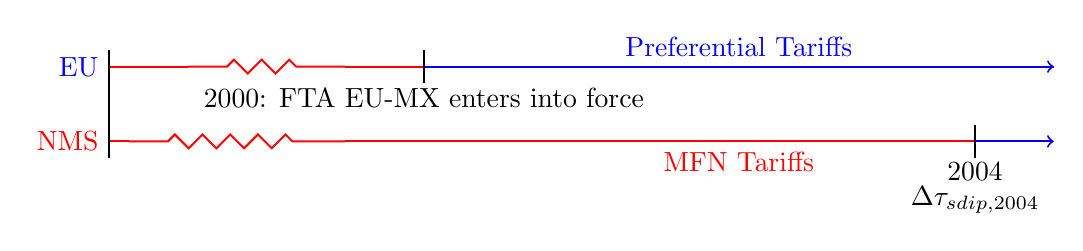
\begin{tikzpicture}[snake=zigzag, line before snake = 5mm, line after snake = 5mm, line width=0.25mm]
  % draw horizontal line   
  \draw[red] (0,0) -- (.25,0);
  \draw[red,snake] (.25,0) -- (3,0);
  \draw[red] (3,0) -- (4,0);
  \draw[red] (4,0) -- (11,0);
  \draw[blue,->] (11,0) -- (12,0);


  \draw[red] (0,.95) -- (1,.95);
  \draw[red,snake] (1,.95) -- (3,.95);
  \draw[red] (3,.95) -- (4,.95);
  \draw[blue] (4,.95) -- (12,.95);
  \draw[blue,->] (11,.95) -- (12,.95);

  % draw vertical lines
  \foreach \x in {11}
    \draw (\x cm,.205) -- (\x cm,-.205);
  \foreach \x in {4}
    \draw (\x cm,{.95+(.205)}) -- (\x cm,{.95-(.205)});
  \foreach \x in {0}
    \draw (\x cm,{.95+(.205)}) -- (\x cm,{0-(.205)});

  % draw nodes
  \draw (8,0.95) node[below=.105] {} node[above=.105] {} node[above=.105] {\textcolor{blue}{Preferential Tariffs}};
  \draw (0,0) node[below=.105] {}  node[left=.105] {\textcolor{red}{NMS}};
  \draw (0,0.95) node[below=.105] {} node[above=.105] {} node[left=.105] {\textcolor{blue}{EU}};
  \draw (4,.95) node[below=.5] {} node[above=.105] {} node[below=4] {2000: FTA EU-MX enters into force};
  \draw (11,0) node[below=.105] {} node[above=.105] {} node[below=4] {2004};
  \draw (11,-.3) node[below=.105] {} node[above=.105] {} node[below=4] {$\Delta \tau_{sdip,2004}$};
  \draw (8,0) node[below=.105] {} node[above=.105] {} node[below=.105] {\textcolor{red}{MFN Tariffs}};
\end{tikzpicture}

\end{document}